\documentclass{article}

% Language setting
% Replace `english' with e.g. `spanish' to change the document language
\usepackage[english]{babel}

% Set page size and margins
% Replace `letterpaper' with `a4paper' for UK/EU standard size
\usepackage[letterpaper,top=2cm,bottom=2cm,left=3cm,right=3cm,marginparwidth=1.75cm]{geometry}

% Useful packages
\usepackage{amsmath}
\usepackage{graphicx}
\usepackage[colorlinks=true, allcolors=blue]{hyperref}
\usepackage{xcolor}
\usepackage{datetime}
\usepackage[section]{placeins} 
\usepackage{pdfpages}
\usepackage{float}

\title{ME136 Lab 2}
\author{Nathan Yacovetta, Aarchan Saxena, Jobanpreet Mutti, Radhika Marolia}
\date{October 5, 2023}

\begin{document}
\maketitle

\section{Contributions}

\begin{itemize}
\item Nathan Yacovetta: Performed lab tasks and implemented lab code, and worked on graphs for 1B, the denoising of signals, and the write up for 3.4 and 3.5. 
\item Aarchan Saxena: Worked on implementing the pwmCommandFromSpeed, the linear regression for correlating PWM to angular velocity, and did the write up for 3.1 and 3.2.
\item Jobanpreet Mutti: Calculated the Betas, propeller thrusts. De-noised the z accel, plotted the measured speed, plotted the thrust.
\item Radhika Marolia: Worked on data collection, wrote the write-up for 2.1 - 2.3, and formatted the images and code on the write-up.
\end{itemize}

\section{For the PWM-speed map:}

\subsection{Part A}

The plot showing the commanded values and measured speeds:

\begin{figure} [H]
\centering
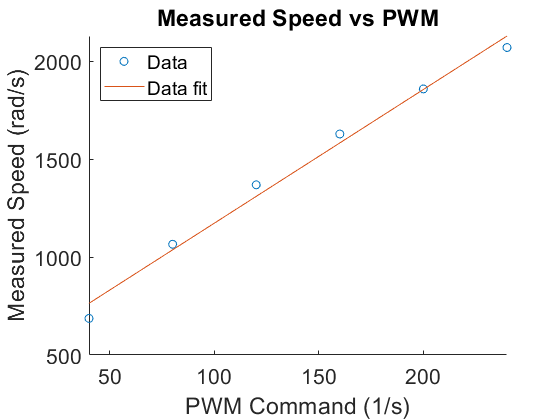
\includegraphics[scale=.65]{2aPNG.png}
\caption{Measured Speed Versus PWM \label{fig1}}
\end{figure}
\FloatBarrier
\vspace{24pt}
\subsection{Part B}

We used a linear regression fit because the data appears to follow a mostly linear shape. This is because the amount of power input going in is linearly related to the angular speed of the motor.

Our code for this implementation is below:

\begin{figure} [H]
\centering
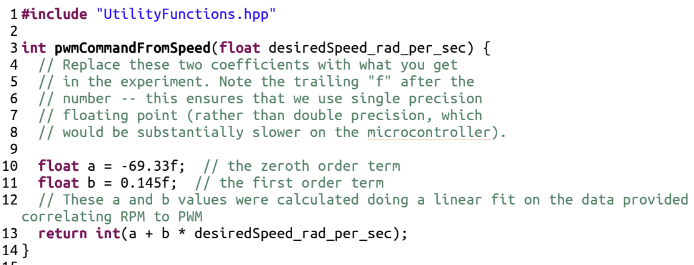
\includegraphics[scale=.65]{me136lab2Q2b.png}
\caption{Code listing of our function implementation from UtilityFunctions.cpp \label{fig2}}
\end{figure}
\FloatBarrier

\subsection{Part C}
For the linear regression, we had an a value of -69.33 and a b value of 0.145. The a value is the 0th degree term of our linear regression and the b value is the 1st degree term for our linear regression. Since this line of best fit has a small least squares error, it shows that the PWM signal you want is linearly dependent on the motor speed you want to achieve.

\section{For the speed-force map:}

\subsection {Part A}
We had the drone hanging by its side off the edge of a table towards the ground off a rod (off the side of a table) and the accelerometer was fixed on the drone. The initial position of the drone is such that the acceleration due to gravity is applied in the y direction, and the acceleration in the x and z directions is 0\(m/s^2\). As the drone's propellers spin, the drone is lifted up to a constant angle, but is constrained in movement by the string that attaches it to the table.




\subsection {Part B}
Using the different motor commands, we could find the drone's z acceleration. Due to the set up of the experiment, the only acceleration acting on the drone was gravity in the y direction, so \(g = 9.81 m/s^2\), and the acceleration in the z direction was \(0 m/s^2\). The angle of the drone could then be calculated with the measurements of the accelerometer. Using the accelerometer data, the angle \(\beta\) can be calculated starting with the equation \[\alpha = ||g||*sin(\beta)\] In this case, \(||g|| = 9.81 m/s^2\), so \(\beta\) could be calculated to be \[\beta = sin^{-1}\left(\frac{\alpha}{9.81}\right)\]

To find the value of acceleration in the z direction, we waited until the acceleration was constant. We then took the average of the sensor output once it was constant to de-noise the signal and figure out the actual average acceleration.

\subsection {Part C}
The plot showing the commanded speeds and the determined per-motor force:

\begin{figure} [H]
\centering
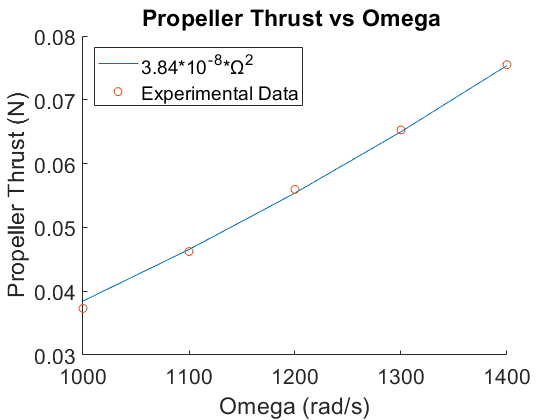
\includegraphics[scale=.90]{PTVSOMEGA.png}
\caption{Propeller Thrust versus Omega \label{3}}
\end{figure}
\FloatBarrier

\subsection {Part D}
Because the thrust equation is a function of omega squared, we can expect our experimental data for thrust to similarly follow a quadratic path. Comparing the theoretical equation with our data highlights this match. The equation for thrust is shown below, and it can be seen that thrust is directly proportional to omega squared.

\[T = C_{T}\cdot p\cdot\Omega^{2}\]
Our code for this implementation is below:

\begin{figure} [H]
\centering
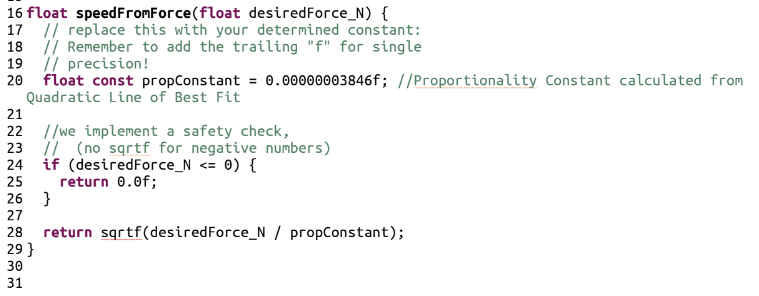
\includegraphics[scale=.65]{me136lab2Q3d.png}
\caption{Code listing of our function implementation from UtilityFunctions.cpp \label{fig2}}
\end{figure}
\FloatBarrier

\subsection {Part E}
Our results closely match the expected thrust equation and all deviations can be attributed to the noise present in the simulation. Our data follows the expectation that acceleration is only present in the y direction. Our data also shows the trend that PWM is linearly related to rotational speed and that this is quadratically related to the thrust produced.

\section{MainLoop Function}

\subsection{Virtual Machine Code}

On the page below is the full listing of our UserCode with comments where we added code to the MainLoop function starting at line 49:
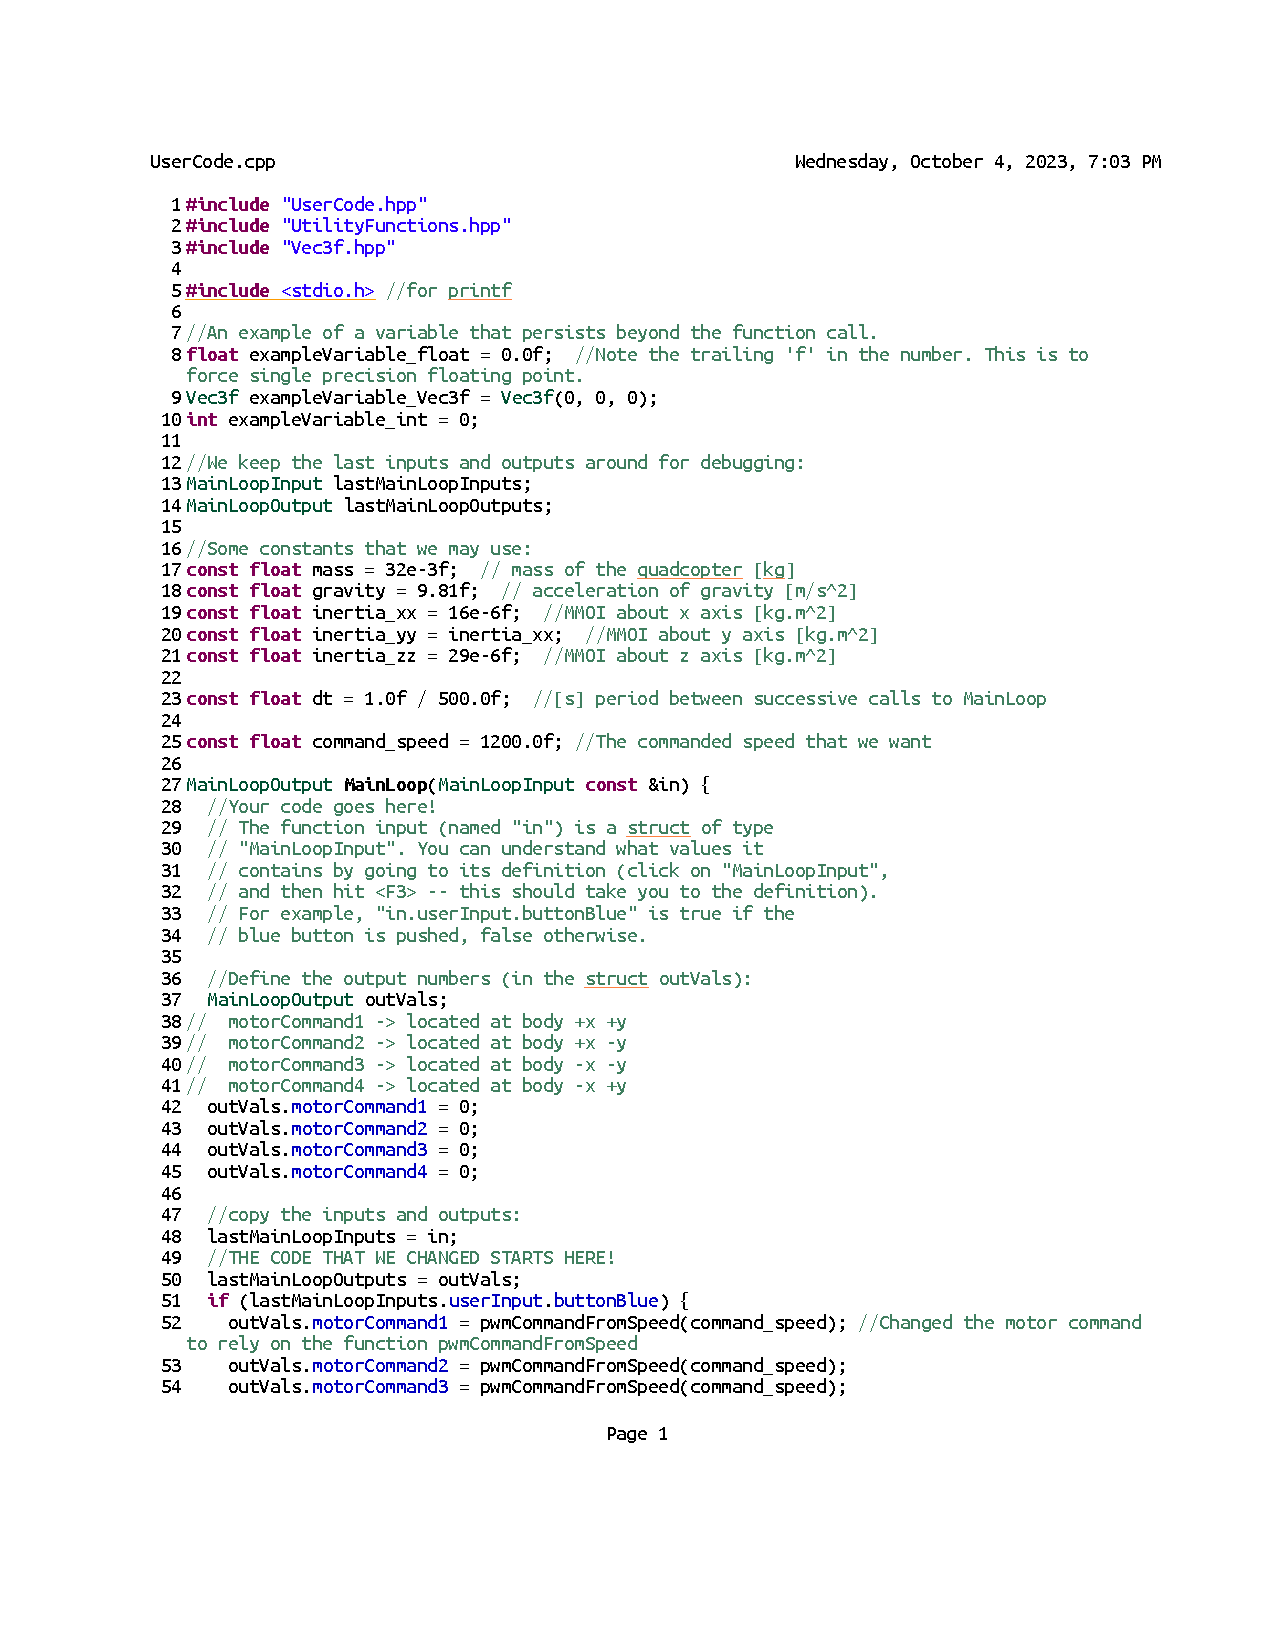
\includepdf[pages=-]{Lab2Usercode.pdf}

On the page below is the full listing of our UtilityCode with comments where we inputed the a and b values and prop constant:
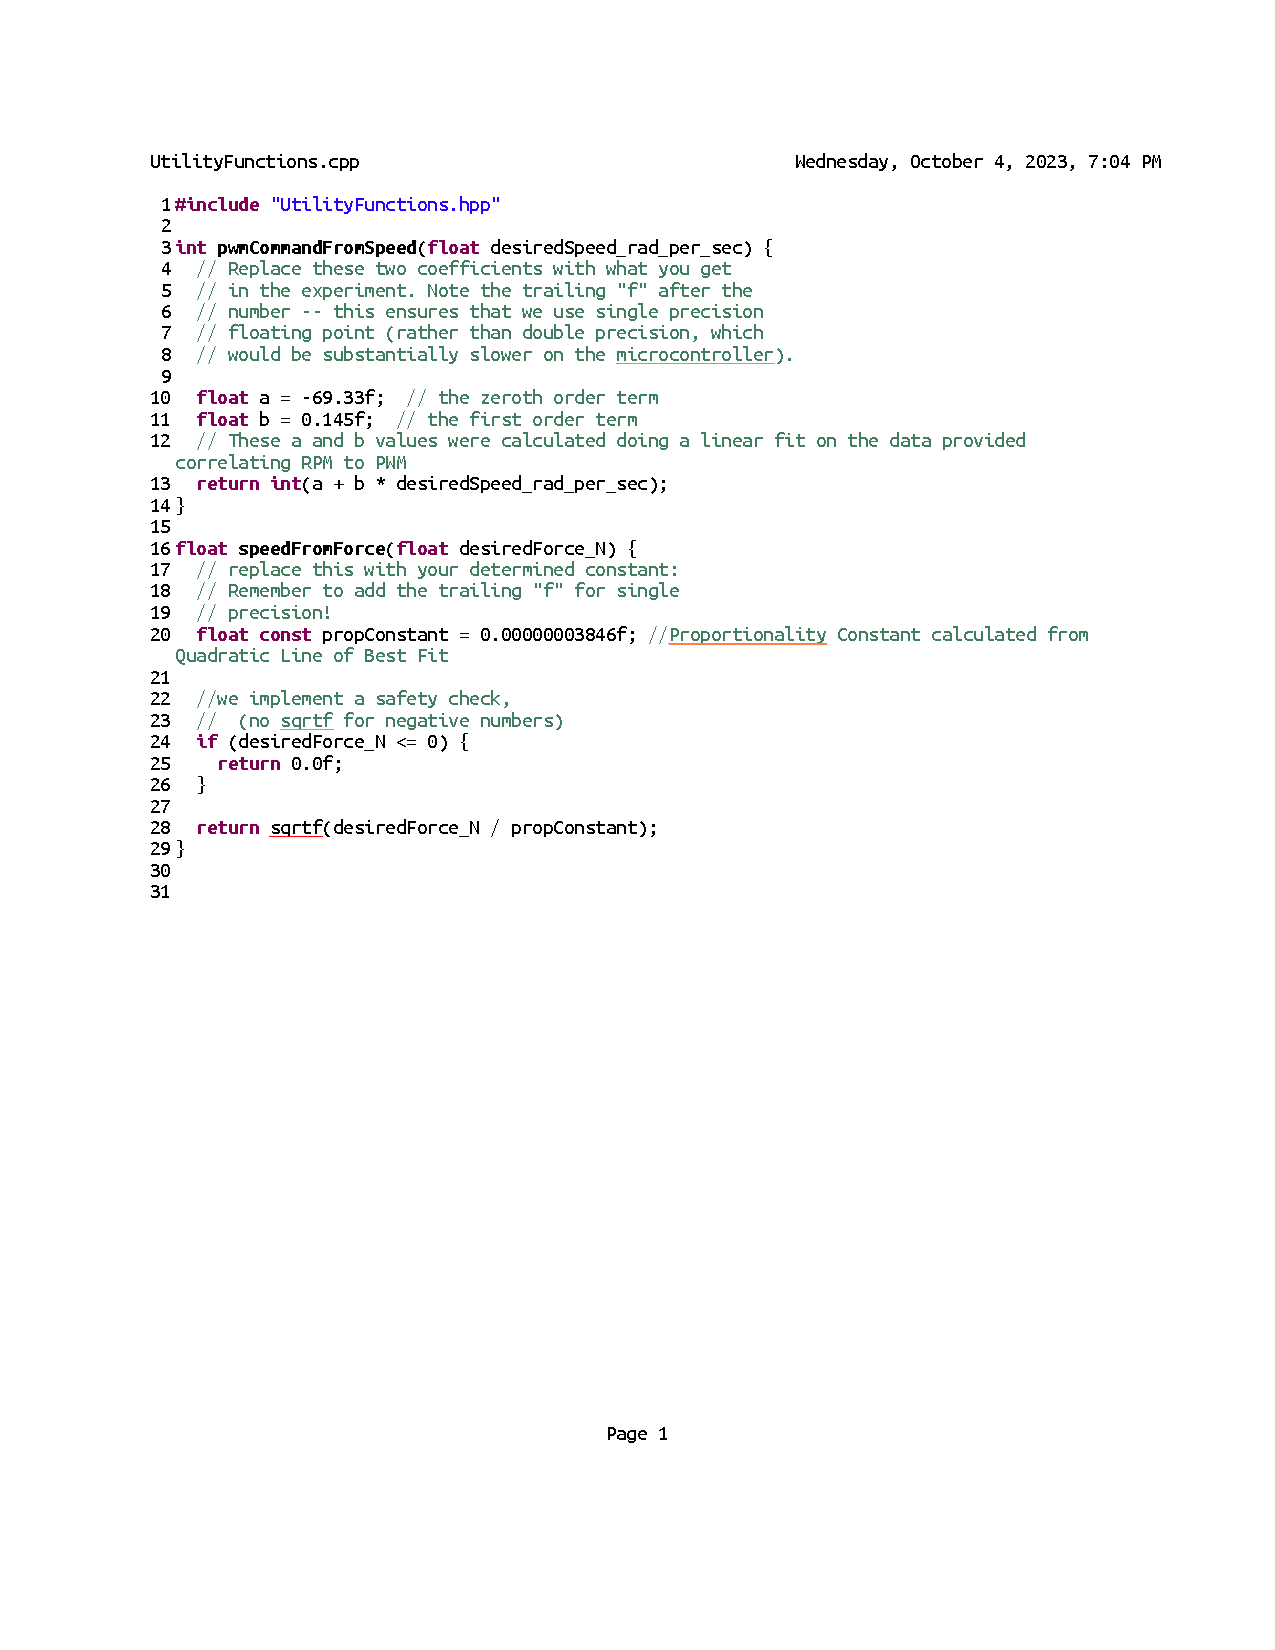
\includepdf[pages=-]{Lab2UtilityCode.pdf}

\subsection{Matlab Code}
On the page below is our Matlab code we used for the linear regression and quadratic fit. This is also where we calculated the force per propeller. It also contains code for 2.3.2 z accel plots:

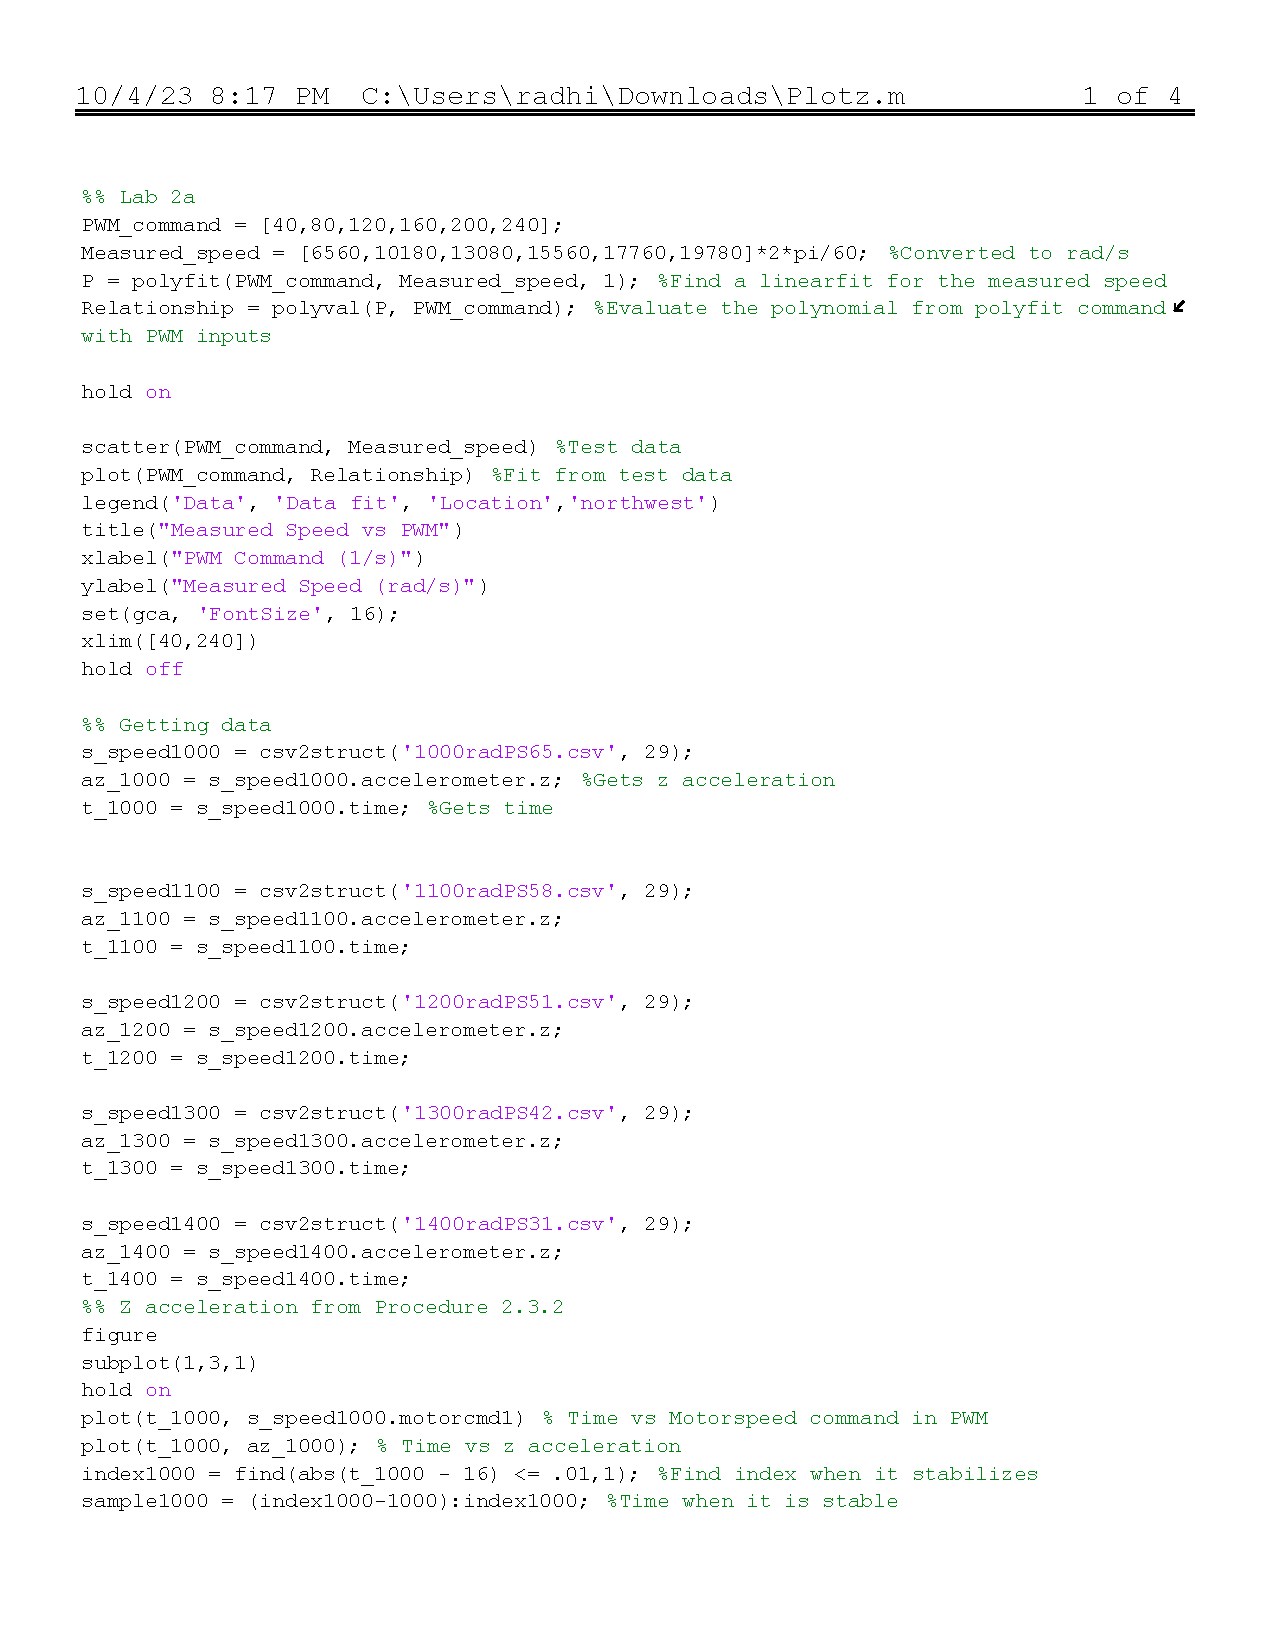
\includepdf[pages=-]{me136lab2matlabcode.pdf}

\end{document}